% Poster v2 — gemini theme with UK blue colors, compiles with lualatex
\documentclass[final]{beamer}

\usepackage[T1]{fontenc}
\usepackage[utf8]{luainputenc}
\usepackage{lmodern}
\usepackage[size=custom,width=122,height=91,scale=1.2]{beamerposter}
\usetheme{gemini}
\usepackage{graphicx}
\usepackage{amsmath,amssymb}
\usepackage{booktabs}
\usepackage{xcolor}
\usepackage{tikz}
\usepackage{anyfontsize}

% ==================
% Override gemini colors with UK blue
% ==================
\definecolor{ukblue}{RGB}{0,51,160}
\definecolor{ukbluedark}{RGB}{0,33,105}
\definecolor{ukbluelight}{RGB}{235,239,250}

\setbeamercolor{headline}{bg=ukbluedark,fg=white}
\setbeamercolor{headline rule}{bg=ukblue}
\setbeamercolor{block title}{bg=ukblue,fg=white}
\setbeamercolor{block separator}{bg=ukblue}
\setbeamercolor{block body}{bg=ukbluelight,fg=black}
\setbeamercolor{footline}{bg=ukbluedark,fg=white}
\setbeamercolor{structure}{fg=ukblue}

% ==================
% Title
% ==================
\title{Message-Passing Graph Neural Network as a Surrogate for Variable-Length 1D Finite Element Bead Chain Simulations}
\author{Grey L.~Goodwin \quad\textbf{\textperiodcentered}\quad Daniel L.~Lau, PhD.}
\footercontent{Department of Electrical and Computer Engineering, University of Kentucky \hfill grey.goodwin@uky.edu}

% ==================
% Column lengths
% ==================
\newlength{\sepwidth}
\newlength{\colwidth}
\setlength{\sepwidth}{0.025\paperwidth}
\setlength{\colwidth}{0.3\paperwidth}
\newcommand{\separatorcolumn}{\begin{column}{\sepwidth}\end{column}}

\begin{document}
\begin{frame}[t]
\begin{columns}[t]
\separatorcolumn

% =============== COLUMN 1 ===============
\begin{column}{\colwidth}

  \begin{block}{Abstract}
    Finite element analysis (FEA) of a flexible bead chain requires
    thousands of force and integration computations per simulated second.
    We train a graph neural network (GNN) to predict the per-timestep
    physics of a 1D bead chain with tapered mass, using randomly sampled
    single-step training data instead of recorded simulations. An initial
    shared MLP achieved accurate predictions on a fixed 16-bead chain but
    could not generalize to other lengths. We restructure the surrogate as
    a true message-passing GNN with separate node/edge encoders, learned
    messages per rod, and ghost masking for endpoints. Because all weights
    are shared, one trained model handles chains of any length.
  \end{block}

  \begin{block}{Problem Setup}
    A whip is modeled as a 1D chain of $N$ tapered mass nodes connected
    by $N-1$ spring rods, anchored at one end. Each free bead experiences
    gravity, Hookean spring forces, rod-axis damping, and velocity drag.
    Time integration uses symplectic Euler:
    \begin{equation}
        \mathbf{v}_i^{n+1} = \mathbf{v}_i^n + \Delta t \, \mathbf{a}(\mathbf{x}^n)
    \end{equation}
    \begin{equation}
        \mathbf{x}_i^{n+1} = \mathbf{x}_i^n + \Delta t \, \mathbf{v}_i^{n+1}
    \end{equation}
    The force on bead $i$ depends only on its state and those of its
    immediate neighbors. This locality is why we use a 1-hop graph
    architecture.
  \end{block}

  \begin{block}{MPGNN Architecture}
    \begin{itemize}
      \item \textbf{Node encoder} $(4 \to 64)$: $[v_x, v_y, m, \text{fixed}]$
      \item \textbf{Edge encoder} $(6 \to 64)$: shared left/right, relative features
      \item \textbf{Message MLP} $(64 \to 64)$: per-edge learned message
      \item \textbf{Ghost mask}: zero messages from absent neighbors
      \item \textbf{Node update MLP} $(192 \to 64)$: fuses self + messages
      \item \textbf{Output head} $(64 \to 4)$: change in state
    \end{itemize}
    80{,}324 parameters, shared across all beads, independent of chain
    length.
  \end{block}

  \begin{block}{Acknowledgements}
    This work was supported in part by the National Science Foundation
    under Grants CCF 2230161 and 2230162 and in part by AFOSR under
    Grant FA9550-22-1-0362.
  \end{block}

\end{column}

\separatorcolumn

% =============== COLUMN 2 ===============
\begin{column}{\colwidth}

  \begin{block}{BeadMPGNN}
    \begin{figure}
      \centering
      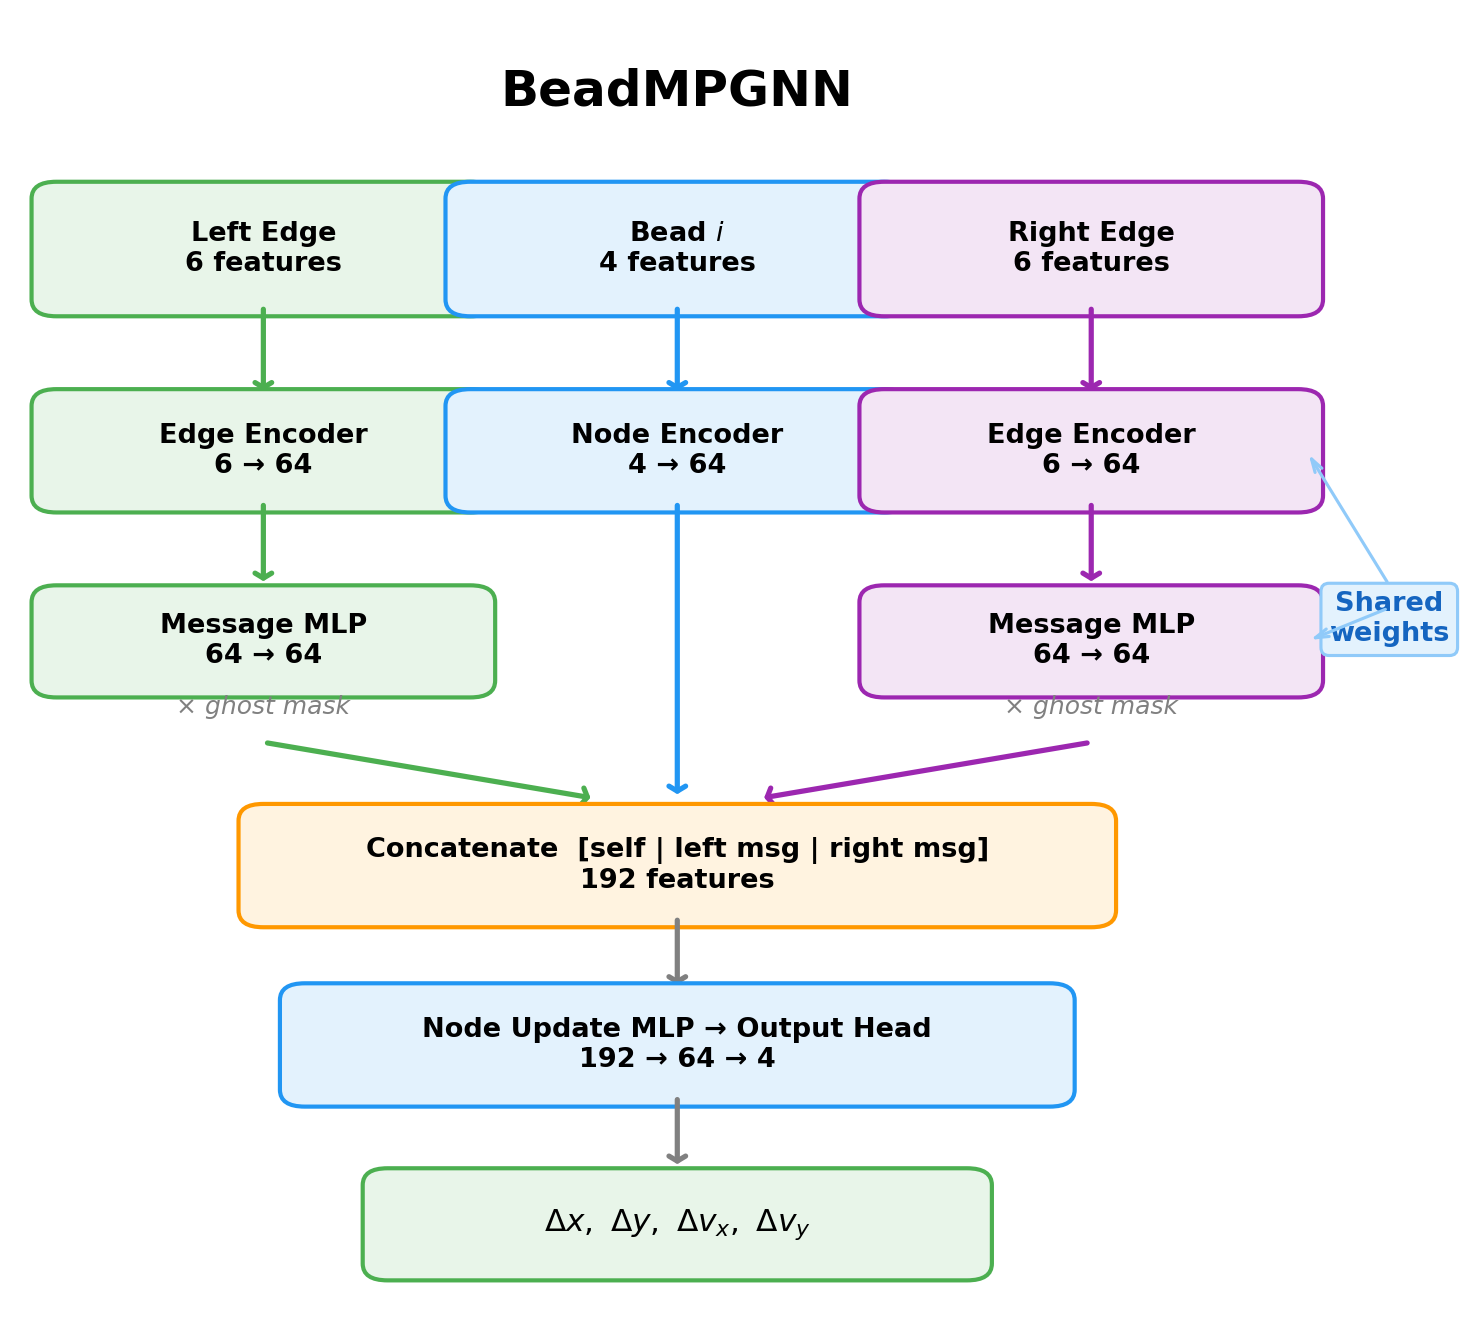
\includegraphics[width=0.8\textwidth]{architecture_mpgnn_only.png}
    \end{figure}
  \end{block}

  \begin{block}{Data Pipeline: Volume Sampling}
    Rather than recording trajectories, we sample random single-step
    scenarios uniformly across the reachable state space. Each sample is
    one bead at one instant plus the exact physics result one timestep later.
    Volume sampling gives the model coverage across the full state space,
    not just along specific trajectories.

    \begin{figure}
      \centering
      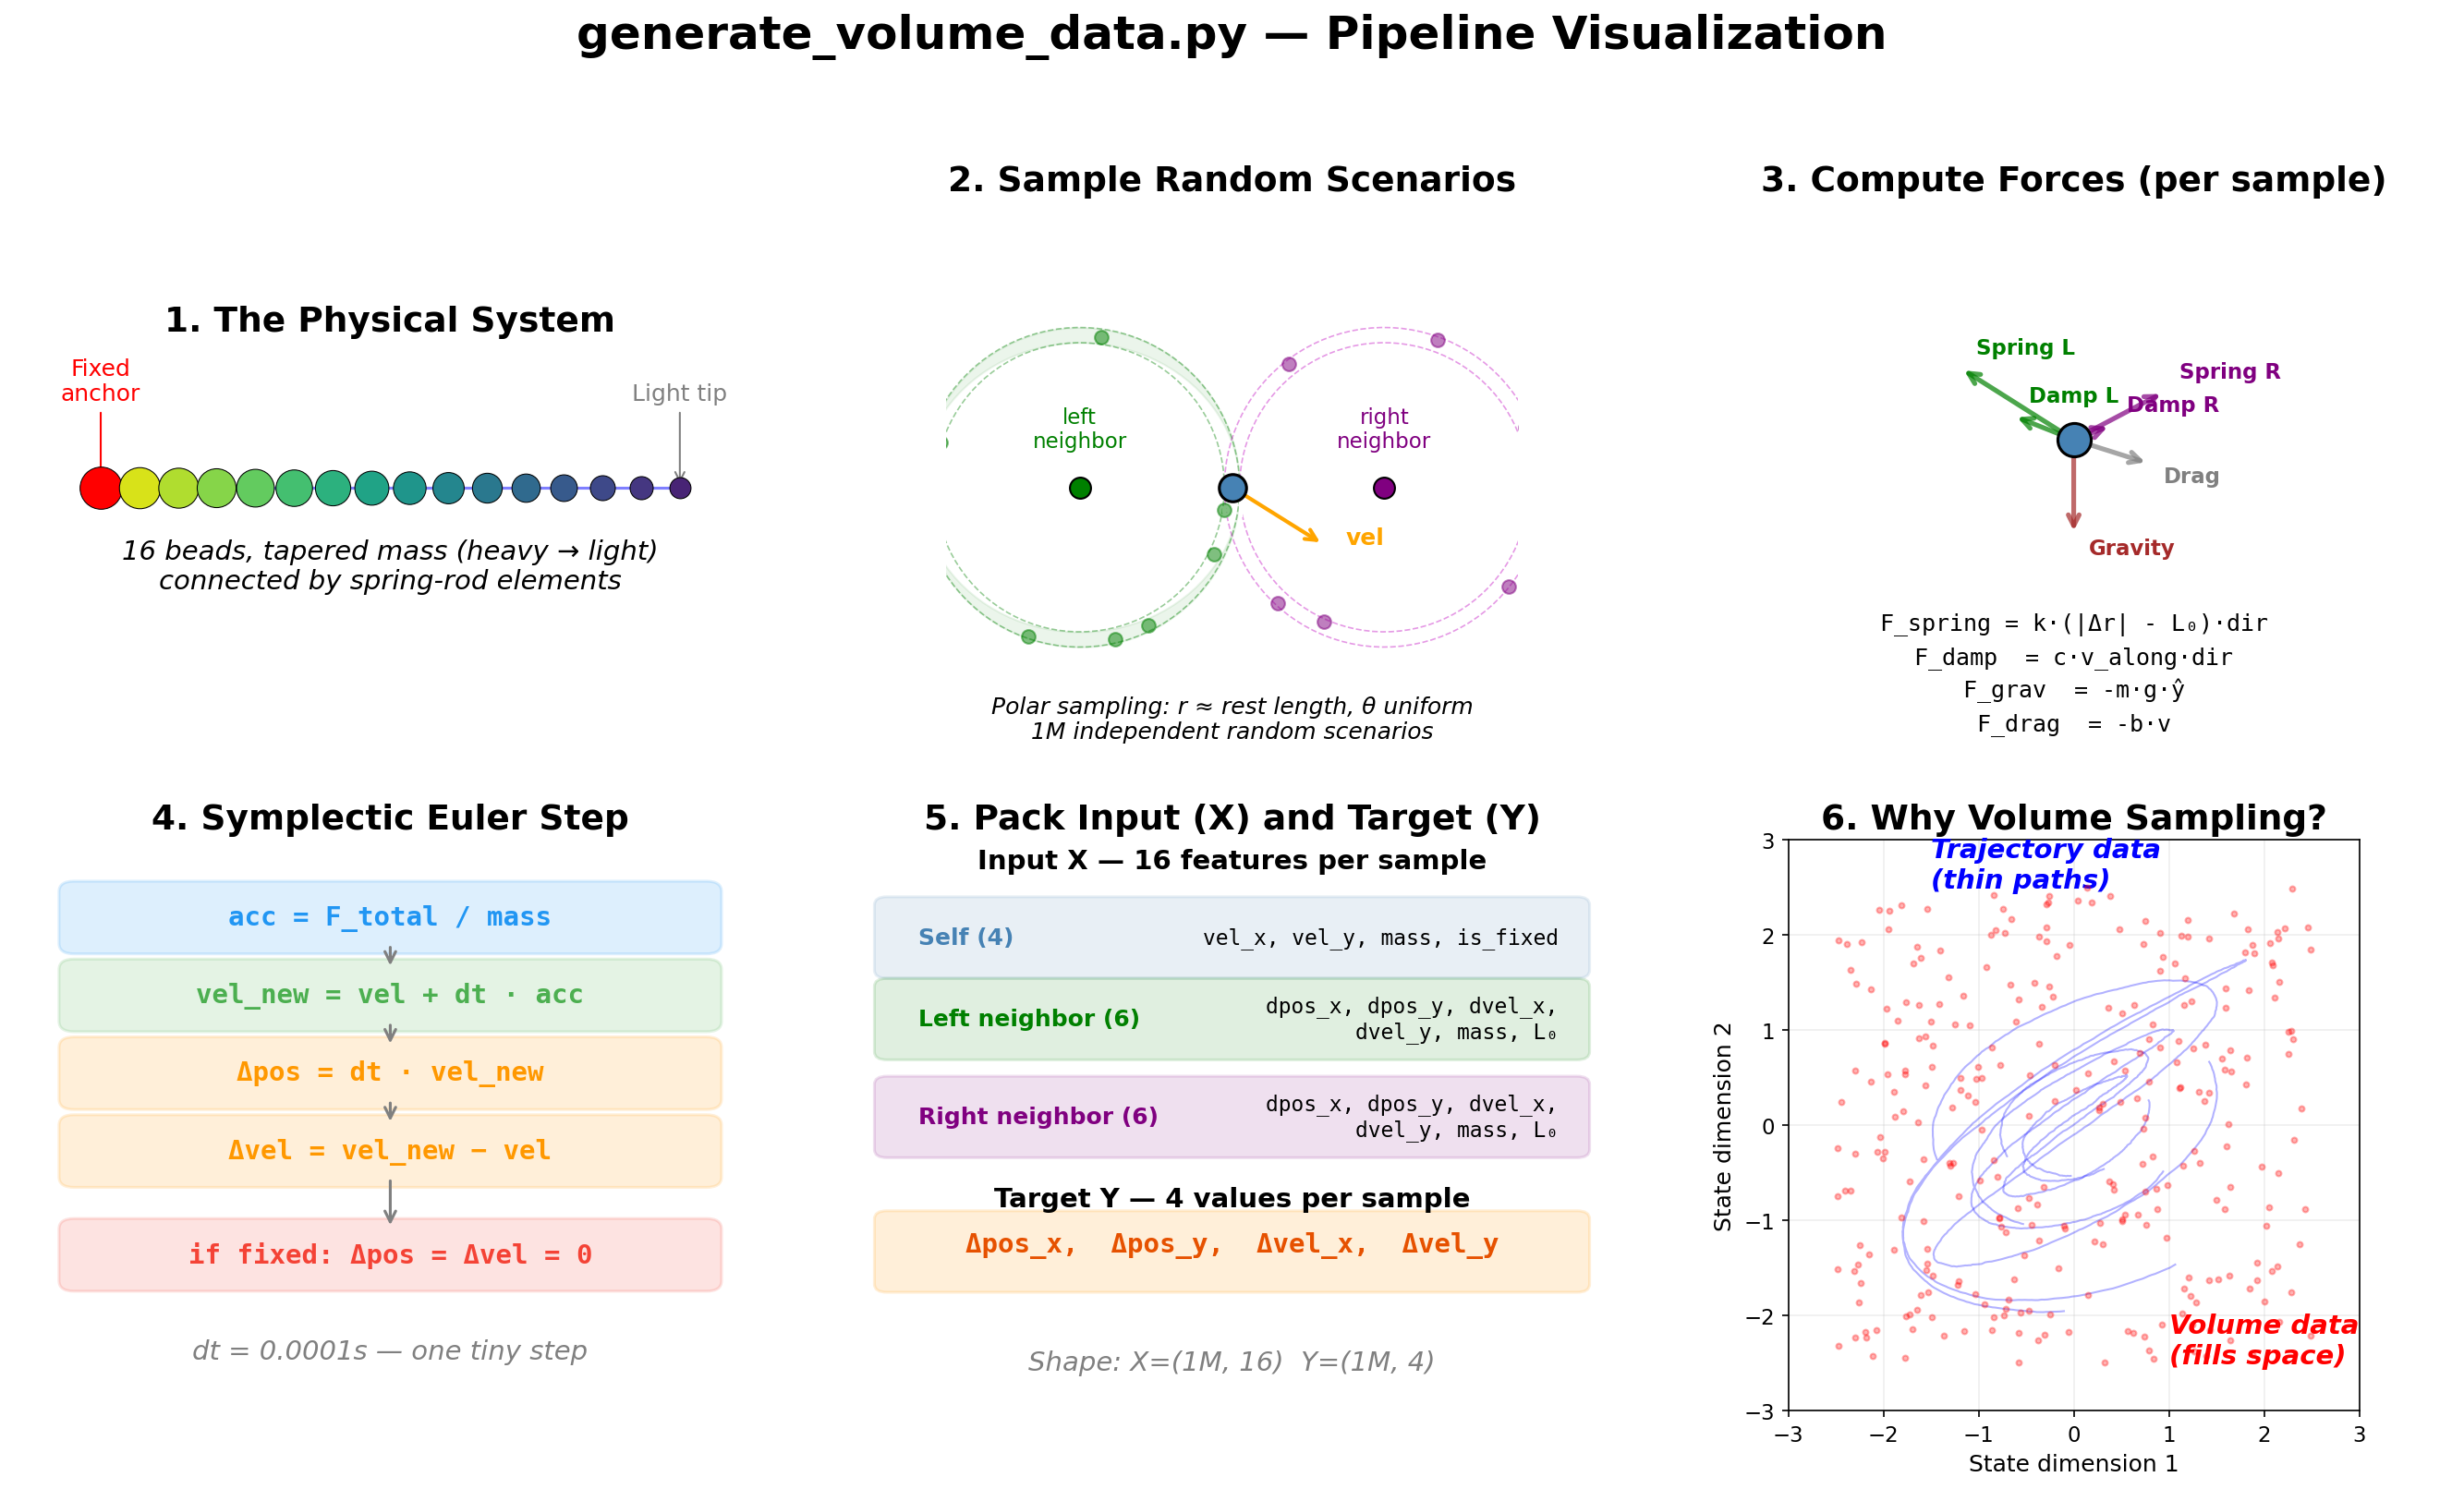
\includegraphics[width=\textwidth]{pipeline_visualization.png}
    \end{figure}
  \end{block}

\end{column}

\separatorcolumn

% =============== COLUMN 3 ===============
\begin{column}{\colwidth}

  \begin{block}{Side-by-Side Rollout}
    \begin{figure}
      \centering
      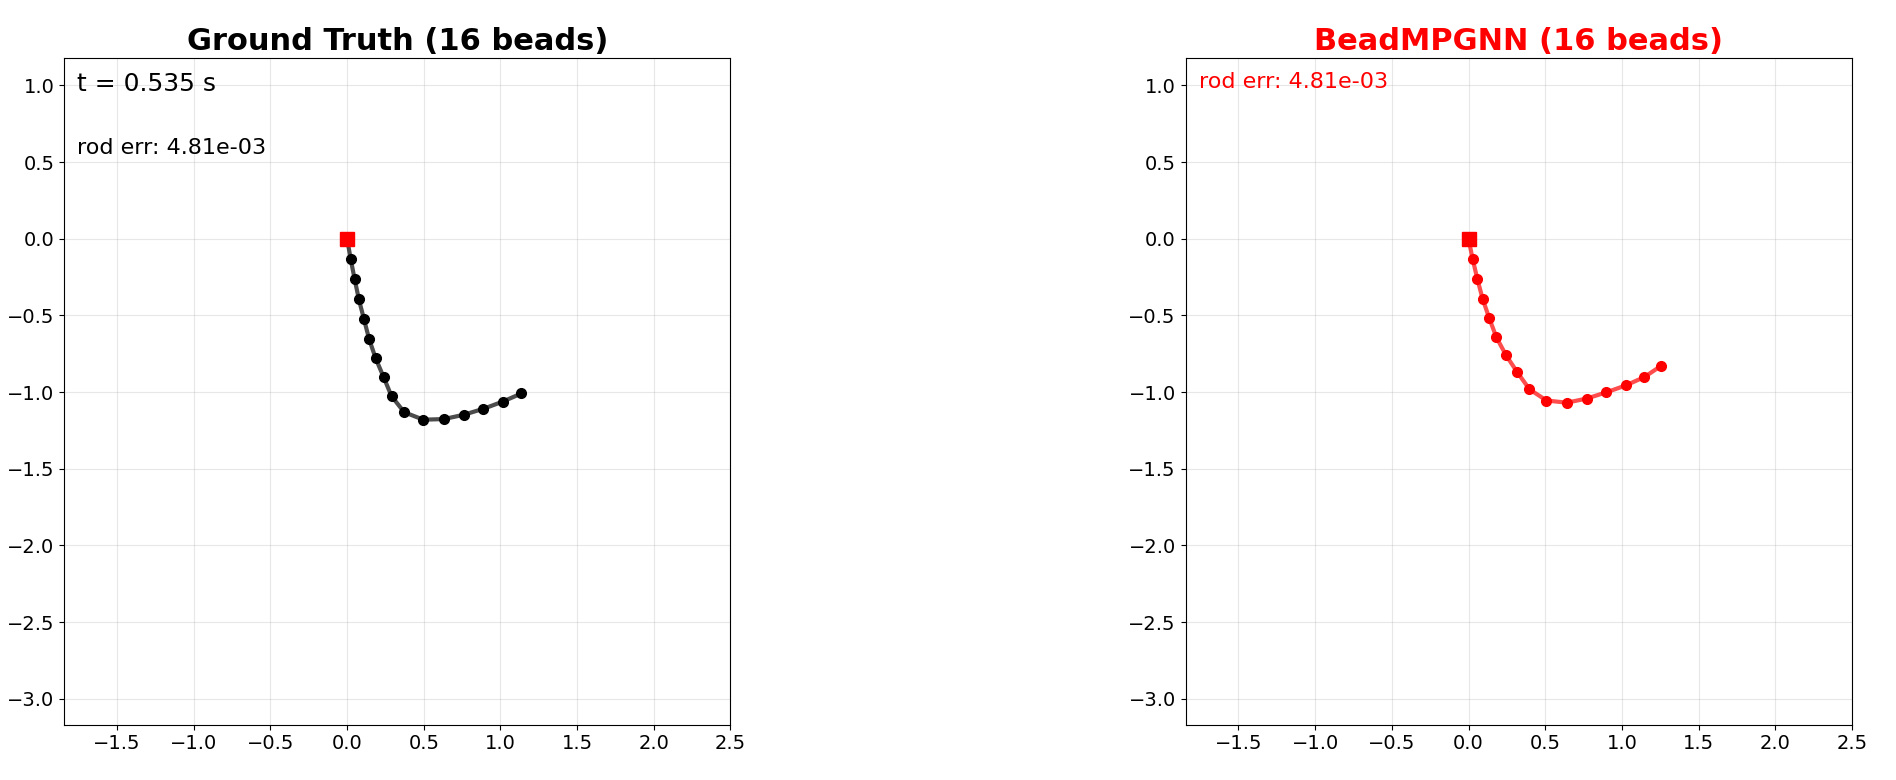
\includegraphics[width=\textwidth]{frame_falling.png}
    \end{figure}
    Ground truth (left, black) vs BeadMPGNN (right, red) on a 16-bead
    chain at $t = 0.535$~s.
  \end{block}

  \begin{block}{Training Convergence}
    \begin{figure}
      \centering
      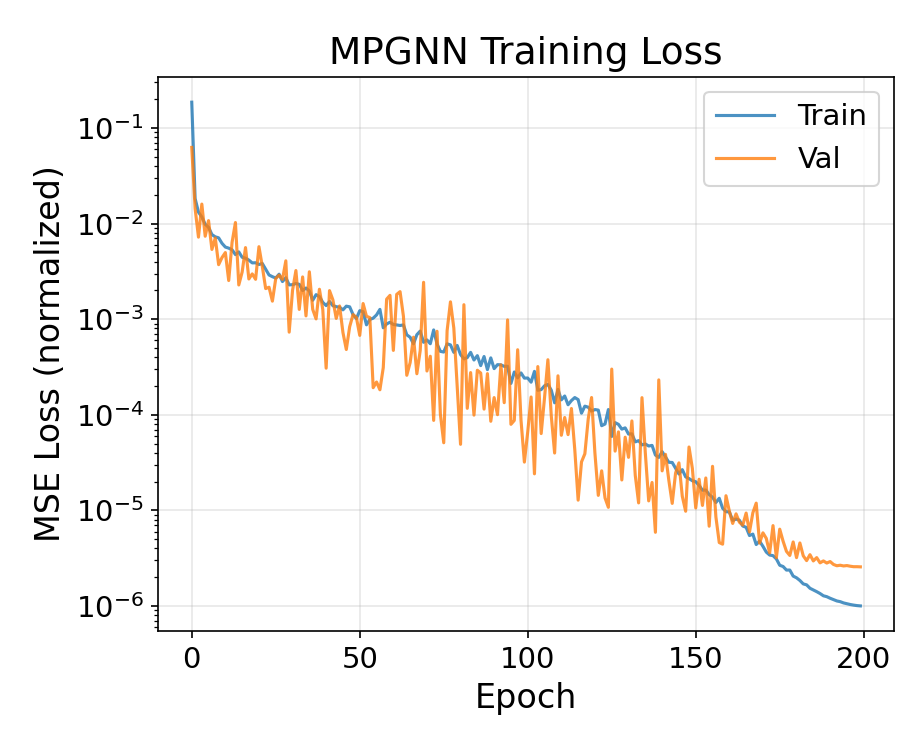
\includegraphics[width=0.8\textwidth]{mpgnn_loss_only.png}
    \end{figure}
  \end{block}

  \begin{block}{Generalization Across Chain Lengths}
    \begin{figure}
      \centering
      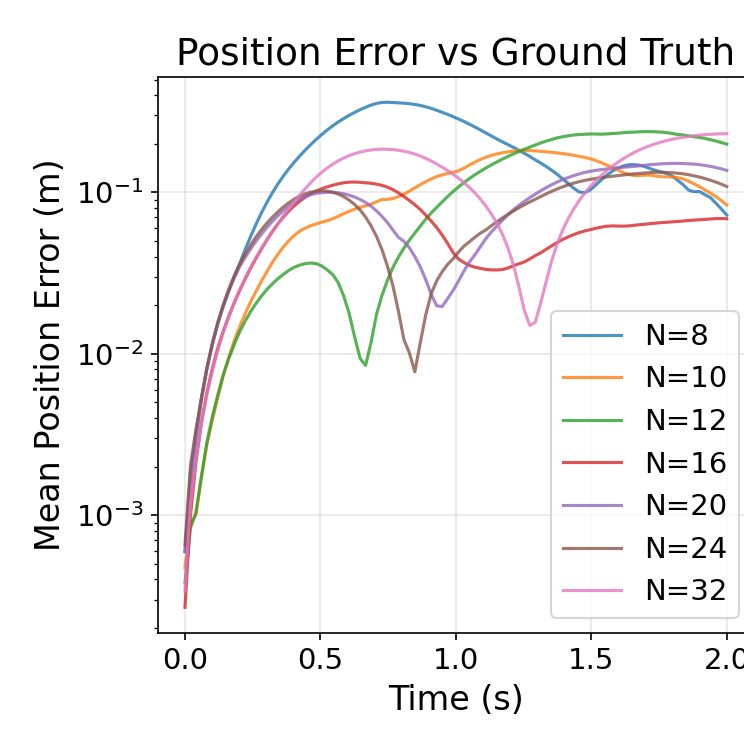
\includegraphics[width=0.8\textwidth]{mpgnn_pos_error_only.png}
    \end{figure}
    Trained on chains of 8--32 beads. Short and medium chains
    ($N \le 16$) track the reference closely. Longer chains
    accumulate more drift.
  \end{block}

  \begin{block}{Conclusion}
    Replacing a fixed-size MLP with a weight-shared message-passing GNN
    lets one trained model simulate bead chains of any length.
    Volume sampling provides the training coverage needed for
    stable rollouts. \textbf{Future work:} rollout training to
    reduce drift.
  \end{block}

\end{column}

\separatorcolumn
\end{columns}
\end{frame}
\end{document}
